\chapter{Результат}

На рисунке \ref{fig:gui} представлен графический интерфейс приложения.

\begin{figure}[H]
	\centering
	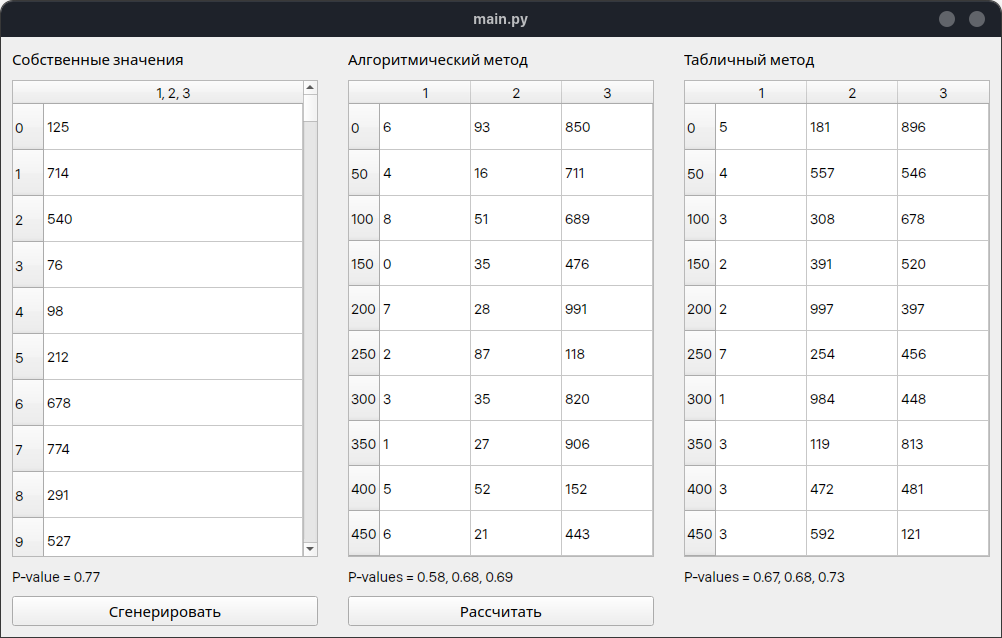
\includegraphics[width=\linewidth]{assets/gui.png}
	\caption{Графический интерфейс приложения}
	\label{fig:gui}
\end{figure}

Программа генерирует последовательность размера 500 чисел.
Заголовки столбцов в таблице обозначают разрядность чисел, представленных в 
этом столбце. Заголовки строк -- номер числа в последовательности. Для алгоритмического 
и табличного метода значения выводятся с шагом 50. Для ручного ввода выводятся все значения.
Таблица для ручного ввода доступна к редактированию.

Кнопка <<Сгенерировать>> заполняет таблицу случайно сгенерированными числами. Кнопка <<Рассчитать>>
выводит на экран значения критериев оценки случайности для каждого столбца таблицы слева направо.

Получившиеся значения представлены под таблицами. Как можно заметить, процент случайности растет с увеличением
количества разрядов.